\documentclass{beamer}
\usetheme{Madrid}
\usepackage[italian]{babel}
\usepackage{amsmath}
\usepackage[T1]{fontenc}
% \usepackage{cancel}
% \usepackage{shadow}
\usepackage{hyperref}
    \hypersetup{colorlinks=true,linkcolor=blue}
\usepackage{graphicx}
\usepackage{multicol}

\newcommand{\figurato}[2]{%
\def\arraystretch{0}\setlength\arraycolsep{1pt}
    \begin{array}[b]{@{}c|c}
        \multicolumn{2}{c}{\rule{0pt}{2pt}}\\\cline{1-1}
        \\[2\arraycolsep]\scriptstyle #1&\smash{\scriptstyle #2}
    \end{array}
}

\title{\textbf{Calcolo del numero delle rate di una rendita posticipata immediata}}
\author{Xianglong Chen}
\date{A.S. 2024/2025}

\begin{document}

\begin{frame}
    \titlepage
\end{frame}

\begin{frame}
    \frametitle{Indice}
    \tableofcontents
\end{frame}

\section{Introduzione teorica}

\begin{frame}
    \frametitle{Introduzione Teorica}
    Nei libri stampati che trattano le rendite finanziarie, è uno spauracchio tipografico condiviso la notazione utilizzata per i coefficienti di commutazione, che utilizzano un simbolo molto poco matematico chiamato \emph{figurato}.
    \[
         a\figurato{n}{i} \hspace{1cm} s\figurato{n}{i} \hspace{1cm} \ddot{a}\figurato{n}{i}  \hspace{1cm} \ddot{s}\figurato{n}{i} 
    \]

    Il primo, impiegato in questa trattazione, si chiama:
    \begin{center}
        <<$a$ figurato $n$, al tasso~$i$>>
    \end{center}
    
\end{frame}

\begin{frame}[fragile]
    \frametitle{Come inserire i coefficienti di commutazione in \LaTeX}

    Con \LaTeX\ è possibile creare un comando apposito:

    \begin{verbatim}
\newcommand{\figurato}[2]{%
\def\arraystretch{0}\setlength\arraycolsep{1pt}%
\begin{array}[b]{@{}c|c}
\multicolumn{2}{c}{\rule{0pt}{2pt}}\\\cline{1-1}
\\[2\arraycolsep]\scriptstyle #1&\smash{\scriptstyle #2}
\end{array}}
    \end{verbatim}

    Da richiamare con la sintassi: \verb|$a\figurato{n}{i}$|
\end{frame}

\section{Dimostrazione della formula}

\begin{frame}
    \frametitle{Relazione Generale}

    Formula iniziale:

    $$ A = R \cdot{a\figurato{n}{i}} $$

    o in forma espansa:
    $$ A = R \cdot \frac{1 - (1+i)^{-n}}{i} $$
\end{frame}

\begin{frame}
    \frametitle{Passaggi Intermedi}

    Moltiplicando per il tasso unitario $i$:
    
    $$ A \cdot i = R \cdot (1 - (1+i)^{-n}) $$
   
    Dividendo per la rata $R$:

    $$ 1 - (1+i)^{-n} = \frac{Ai}{R} $$

    Isolando il termine $(1+i)^{-n}$:
    
    $$ (1+i)^{-n} = 1 - \frac{Ai}{R} $$
\end{frame}

\begin{frame}
    \frametitle{Determinazione dell'incognita $n$}

    Applicando il logaritmo a entrambe i membri:
    
    $$ \ln(1+i)^{-n} = \ln\left(1 - \frac{Ai}{R}\right) $$

    Per la proprietà dei logaritmi che coinvolge le potenze:
    
    $$ -n \ln(1+i) = \ln\left(1 - \frac{Ai}{R}\right) $$

    Isolando definitivamente l'incognita $n$:
    
    \begin{equation}
        \boxed{n = -\frac{\ln\left(1 - \frac{Ai}{R}\right)}{\ln(1+i)}}
        \label{eq:enne}
    \end{equation}
        
    
\end{frame}

\section{Considerazioni teoriche}

\begin{frame}
    \frametitle{Considerazioni Teoriche}

    Il logaritmo e la funzione logaritmica sono definiti solo quando il loro argomento è \emph{strettamente positivo}.\\[1em]

    Nella formula~(\ref{eq:enne}) occorre quindi discutere:

    \[
        1-\frac{Ai}{R} > 0 \quad \Rightarrow \quad R > Ai 
    \]
    


    Dal punto di vista matematico, questa condizione assicura che il logaritmo rimanga sempre definito.

    Dal punto di vista finanziario, la singola rata $R$ deve essere maggiore degli interessi maturati alla prima scadenza, altrimenti \emph{il debito non potrà mai essere estinto}.
\end{frame}

\section{Script Javascript}

\begin{frame}[fragile,shrink=20]
    \frametitle{Script in Javascript (codice)}

    % Codice per calcolare il numero delle rate:
    \setlength{\columnsep}{18cm}
    \begin{multicols}{2}
        
        \begin{verbatim}
<html>
<head>
  <title> Calcolo del numero della rendita posticipata immediata </title>
</head>
<body>
<form name="Dati iniziali">
 <fieldset>
<legend>Dati iniziali</legend>
Importo finanziamento:
<input type="text" name="A" id="A" style="text-align:right;"> € <br><br>
Importo rata:
<input type="text" name="rata" id="rata" style="text-align:right;"> € <br><br>
Tasso (T.A.E.G.):
<input type="text" name="tasso" id="tasso" style="text-align:right;"> % <br><br>
Periodicità dei pagamenti:
<select id="periodo">
 <option value="12">Mensile</option>
 <option value="4">Trimestrale</option>
 <option value="2">Semestrale</option>
 <option value="1">Annuale</option>
</select>
<br>
<br>
<button type="button" onclick="Calcola()"> Calcola </button>
<button type="reset"> Reset </button>
 </fieldset>
</form>

<p id="output_n"></p>
<p id="output_opzione1"></p>
<p id="output_opzione2"></p>

<script>

function Calcola()
{
    var A = parseFloat(document.getElementById("A").value.replace(',', '.'));
    var R = parseFloat(document.getElementById("rata").value.replace(',', '.'));
    var r = parseFloat(document.getElementById("tasso").value.replace(',', '.'));
    var periodo = parseInt(document.getElementById("periodo").value);
   
    if (periodo == 1)
{
      var  i = r / 100;
    }
else
    {
     i = Math.pow(1 + r / 100, 1 / periodo) - 1;
    }

    var n = -Math.log(1 - A * i / R) / Math.log(1 + i);
var n1 = n - (n % periodo);
var n2 = n1+periodo;
var afiguno = (1-Math.pow(1+i,-n1))/(i);
var afigdue = (1-Math.pow(1+i,-n2))/(i);
var erreuno = A/afiguno;
var erredue = A/afigdue;

document.getElementById("output_n").innerHTML = 
"Numero di rate: " + n.toFixed(3);

if (n1/periodo == 1)
{document.getElementById("output_opzione1").innerHTML = 
"Prima opzione: finanziamento a "+n1/periodo+" anno ("+ n1+" rate) 
dell'importo pari a "+ erreuno.toFixed(2)+" € ciascuna";
}
else
{
document.getElementById("output_opzione1").innerHTML = 
"Prima opzione: 
finanziamento a "+n1/periodo+" anni ("+ n1+" rate)
dell'importo pari a "+ erreuno.toFixed(2)+" € ciascuna";
}
document.getElementById("output_opzione2").innerHTML =
"Seconda opzione: finanziamento a "+n2/periodo+" anni (" + n2+" rate) 
dell'importo pari a "+ erredue.toFixed(2)+" € ciascuna";


}
</script>
</body>
</html>

        \end{verbatim}
    \end{multicols}
\end{frame}

    \begin{frame}{Risultato}
    \frametitle{Visualizzazione del risultato in Browser}
    \begin{figure}
        \centering
        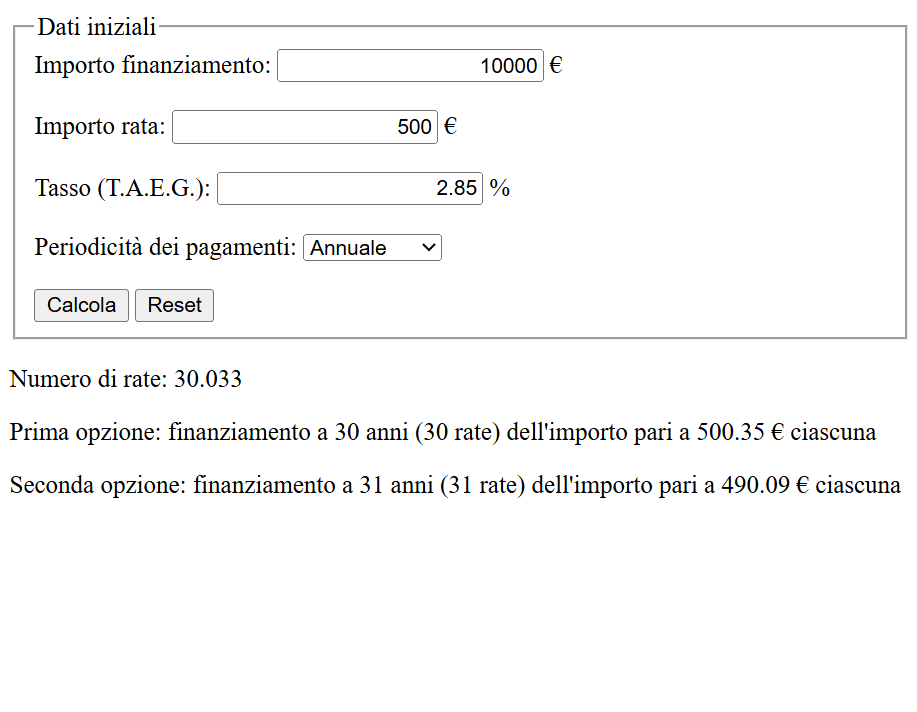
\includegraphics[width=0.7\linewidth]{Risultato_Finale.png}
    \end{figure}
    \end{frame}

    % \begin{frame}
    % \href{file://servereinaudi/STUDENTI/chen.x/Desktop/Matematica%20Finanziaria/n.html}{\beamergotobutton{Link}}
    % \end{frame}


\end{document}
